% 2006 上海理科卷 Q19；四棱锥及底面对角线为矢量示意，不按比例。
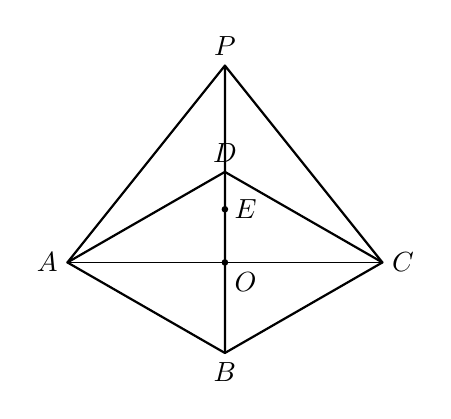
\begin{tikzpicture}[line cap=round,line join=round]
  \coordinate (A) at (-2,0);
  \coordinate (B) at (0,-1.15);
  \coordinate (C) at (2,0);
  \coordinate (D) at (0,1.15);
  \coordinate (O) at (0,0);
  \coordinate (P) at (0,2.5);
  \coordinate (E) at (0,0.675); % PB 的中点

  \draw[thick] (A)--(B)--(C)--(D)--cycle;
  \draw (A)--(C);
  \draw[dashed] (B)--(D);
  \draw[thick] (P)--(A) (P)--(B) (P)--(C) (P)--(D);
  \draw[dashed] (P)--(O);

  \fill (O) circle[radius=1.2pt];
  \fill (E) circle[radius=1.2pt];
  \node[above] at (P) {$P$};
  \node[left] at (A) {$A$};
  \node[below] at (B) {$B$};
  \node[right] at (C) {$C$};
  \node[above] at (D) {$D$};
  \node[below right] at (O) {$O$};
  \node[right] at (E) {$E$};
\end{tikzpicture}
